\documentclass[10pt]{exam}
\usepackage[hon]{template-for-exam}
\usepackage{enumitem,multicol,multirow,tikz,fancybox,graphicx}
\usetikzlibrary{shadings,decorations.pathmorphing,arrows.meta,patterns,calc}
\setlist[enumerate,itemize]{topsep=0pt,itemsep=-1ex,partopsep=1ex,parsep=1ex}

\title{Car Lab \#1}
\author{Rohrbach}
\date{\today}

\begin{document}
\maketitle

\section*{Purpose}

To determine the ways in which a position graph represents an object's motion.

\section*{Materials}

\begin{itemize}
  \item Pick up one blue car and one red car
  \item Pick up a dry erase marker and an eraser
  \item Pick up meter stick 
  \item	Pick up a timer
\end{itemize}

\section*{Procedure}

% Each group has a slightly different experiment:

%   \paragraph{Group 1}	Red car, moving forward, starting at zero
%   \paragraph{Group 2}	Blue car, moving forward, starting at zero
%   \paragraph{Group 3}	Red car, moving backward, starting at 4 meters
%   \paragraph{Group 4}	Red car, moving backward, starting at 2 meters
%   \paragraph{Group 5}	Red car, moving forward, starting at 3 meter
%   \paragraph{Group 6}	Red car, moving backward, starting at 5 meters
%   \paragraph{Group 7}	Red car, moving forward, starting at 1 meter
%   \paragraph{Group 8}	Blue car, moving forward, starting at 2 meters

Before you get started, measure the time it takes each car to travel 1.00~meter.  Record the time and calculate the velocity of each car using the equation $v=\Delta x/\Delta t$.

\begin{multicols}{2}
  \begin{tabular}{|l|c|}
    \hline
    \multicolumn{2}{|l|}{\bf Red Car} \\\hline
    Time to travel 1.00 m (s) &
    Velocity (m/s) \\\hline
    & \\[1em]\hline
  \end{tabular}

  \begin{tabular}{|l|c|}
    \hline
    \multicolumn{2}{|l|}{\bf Blue Car} \\\hline
    Time to travel 1.00 m (s) &
    Velocity (m/s) \\\hline
    & \\[1em]\hline
  \end{tabular}
  
\end{multicols}

\noindent
When you are ready to start the experiment:

\begin{enumerate}
  \item Make a ``track'' that is 5~meters long.  Draw a line and label at ``0~m,'' ``1~m,'' ``2~m,'' ``3~m,'' ``4~m,'' and ``5~m.''
  \item Put the car at 0~m.
  Count down, release the car, and have the timer start calling out the time every 2~seconds.
  \item Every 2 seconds for 12 seconds, make a mark at the location of the car.
  \item Once the car has finished its trip, measure each 2-second mark relative to the zero point.
  \item Repeat 3 times
  \item Repeat for the other car
\end{enumerate}

\section*{Data}

\renewcommand{\arraystretch}{1.6}

\def\cw{.15\textwidth}
\newcommand{\datatable}[2]{
  \def\expno{#1}
  \def\exptitle{#2}
  \begin{center}
    \begin{tabular}
      {
        |*{4}{>{\centering\arraybackslash}m{\cw}|}
        |>{\centering\arraybackslash}m{\cw}|
      }
      \hline
      \multicolumn{5}{|l|}{\textbf{Experiment \expno:} \exptitle} \\
      \hline
      \multirow{2}{\cw}
        {\centering Time (s)} & 
      \multicolumn{4}{c|}{Displacement (m)} \\
      \cline{2-5}
      & Trial \#1 & Trial \#2 & Trial \#3 & Average \\
      \hline  
      2 &&&&\\
      \hline
      4 &&&&\\
      \hline
      6 &&&&\\
      \hline
      8 &&&&\\
      \hline
      10 &&&&\\
      \hline
      12 &&&&\\
      \hline
    \end{tabular}
  \end{center}
}
  
  \datatable{\#1}{Red Car}

  \datatable{\#2}{Blue Car}



\section*{Analysis}
Make a graph on Desmos of your two data sets \textbf{Time be $x$, Average displacement be $y$.}  Plot a best fit line.  Write down the equation for each of the best fit lines below.  You should also copy the link to your graph, paste it on Schoology, and include the link here.


    \vspace{1em}

    Equation for Red Car:

    \vspace{1em}

    Equation for Blue Car:

    \vspace{1em}

    Link to graph: \texttt{https://www.desmos.com/calculator/}\fillin[][15em]


    \vspace{2em}

\vs

\begin{Sbox}\begin{minipage}{6.3in}
\subsection*{How to Graph on Desmos}

Go to \texttt{www.desmos.com/calculator} to graph your data. 

\begin{multicols}{2}

  \begin{enumerate}[label=\alph*),topsep=0pt,itemsep=-1ex,partopsep=1ex,parsep=1ex]
    \item \label{table} Start by making a table by clicking the “+” icon at the top left.  You will need to create two separate tables.
    \item \label{wrench} Make sure to label the axes using the wrench icon at the right.
    \item \label{zoom} Zoom out so that you can see the whole graph and so that it fills the page.  You can do this using the ``Zoom Fit'' option, but be careful that your fit does not cut off one of the graphs
    \item \label{linear} Create best fit lines for each graph using the ``Linear Regression'' tool
    \item Copy a link to your graph using the export button and clicking ``Share a Snapshot''.  Write down the link to this graph so you and your instructor can both access your work, later.
  \end{enumerate}

  \vspace{4em}

  \begin{tikzpicture}
    \node[anchor=north west] at (0,0) 
      {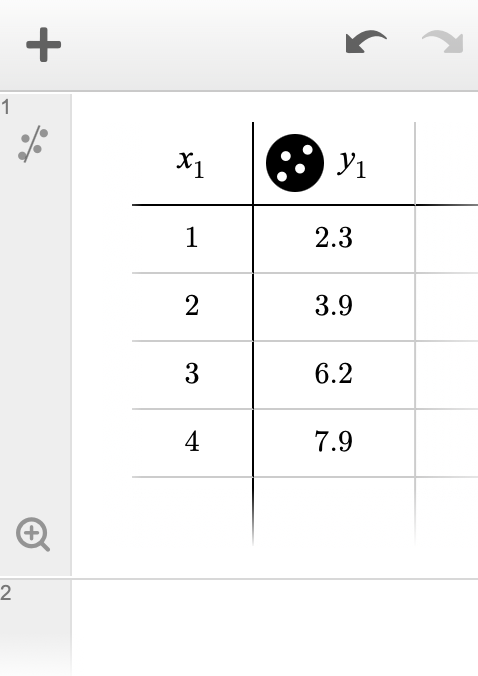
\includegraphics[width=3cm]{desmos1}};


    \node[anchor=north west] at (3.5,0) 
      {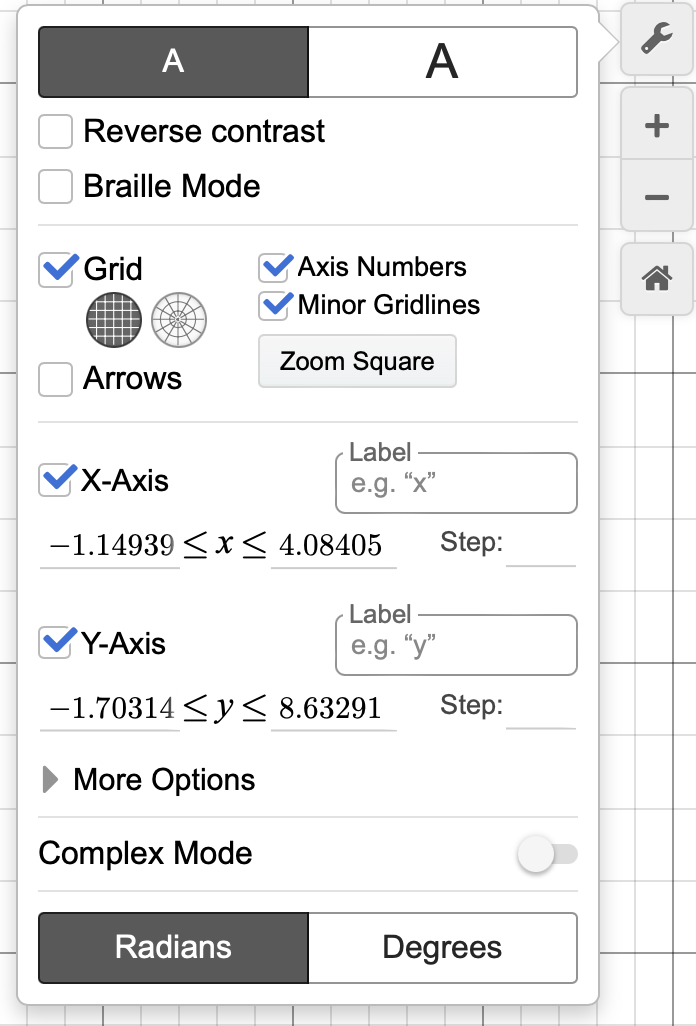
\includegraphics[width=3.5cm]{desmos2}};

        \draw (2,0) 
      node[fill=red!20,rounded corners] (table)
      {\ref{table} Create a table};
    \draw[red] (0.4,-.4) coordinate (a) circle (0.3);
    \draw[<-,red,very thick] (a) +(0.3,0) -- (table.south);

    \node[fill=blue!20,rounded corners] at (2.5,-1.5) (linear) {\ref{linear} Linear Regression};
    \draw[blue] (0.3,-1) coordinate (a) circle (0.3);
    \draw[<-,blue,very thick] (a) +(0.3,0) -- (linear.north);

    \node[fill=green!20,rounded corners] at (2,-2.5) (zoom) {\ref{zoom} Zoom Fit};
    \draw[green, ultra thick] (0.3,-3.5) coordinate (a) circle (0.3);
    \draw[<-,green,very thick] (a) +(0.3,0) -- (zoom.west);

    \node[fill=orange!20,rounded corners] at (4.5,-0.5) (wrench) {\ref{wrench} Axis Labels};
    \draw[orange, ultra thick] (6.9,-.3) coordinate (a) circle (0.3);
    \draw[<-,orange,very thick] (a) +(-0.3,0) -- (wrench.east);

    \draw[->,orange,very thick] (wrench.south) -- (5.2,-2.3);

    \draw[orange, ultra thick, rounded corners] (3.8,-2.3) rectangle ++(2.8,-0.5);
    \draw[orange, ultra thick, rounded corners] (3.8,-3.1) rectangle ++(2.8,-0.5);
  \end{tikzpicture}

\end{multicols}
\end{minipage}\end{Sbox}

\noindent
\shadowbox{\TheSbox}

\pagebreak
\noindent
Write a paragraph explaining what you did on this part of the lab.  Your paragraph should address: (1) what you graphed and what the graph looked like, (2) why the shape of the graph makes sense, and (3) what the physical meaning is of the \emph{slope} and the \emph{y-intercept}.

\pagebreak

\section*{Conclusion}

You calculated the velocity of each car on the first page.  Compare the velocities with the slopes you calculated for each car by calculating a percent error.
%
\begin{align*}
  \text{Percent Error} = \frac{\left| \text{measured} - \text{expected}  \right|}{\text{expected}} \times 100\%
\end{align*}
%
Calculate the percent error and then write a paragraph commenting on your percent error.  Your paragraph should address: (1) How reasonable is your percent error? (2) Identify three to four factors that could have created uncertainties in your measurements and explain how each factor may have influenced your percent error. (3) What can you say you learned about the position graphs of objects and how they are related to the motion of those objects?


\vspace{1em}

Percent Error (Red Car): \fillin[][10em]
%
\hfill
%
Percent Error (Blue Car): \fillin[][10em]



\end{document}